\hypertarget{interfaceBool}{
\section{Bool  Interface Reference}
\label{interfaceBool}\index{Bool@{Bool}}
}
Inheritance diagram for Bool:\begin{figure}[H]
\begin{center}
\leavevmode
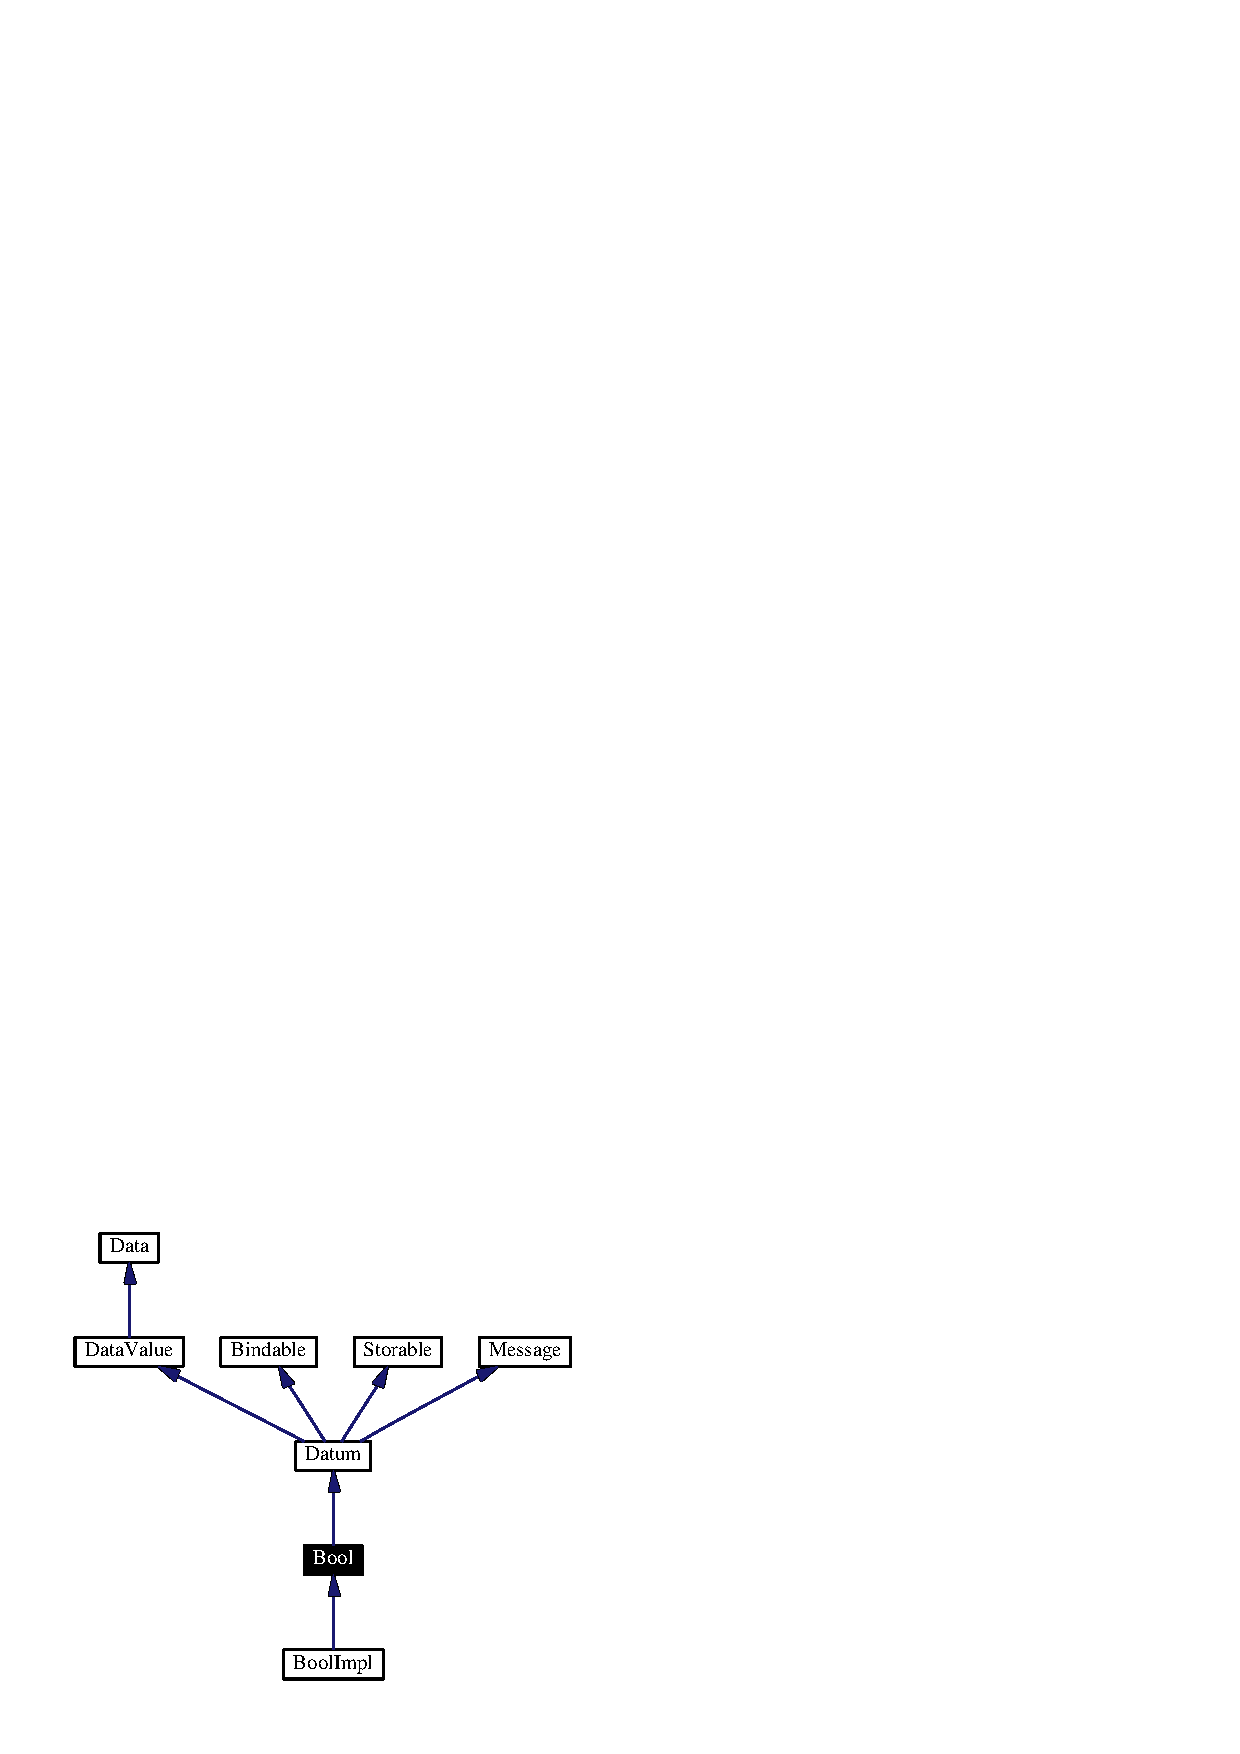
\includegraphics[width=137pt]{interfaceBool__inherit__graph}
\end{center}
\end{figure}
Collaboration diagram for Bool:\begin{figure}[H]
\begin{center}
\leavevmode
\includegraphics[width=137pt]{interfaceBool__coll__graph}
\end{center}
\end{figure}
\subsection*{Public Methods}
\begin{CompactItemize}
\item 
boolean \hyperlink{interfaceBool_a0}{boolean\-Value} ()
\item 
Bool \hyperlink{interfaceBool_a1}{not} ()
\end{CompactItemize}


\subsection{Member Function Documentation}
\hypertarget{interfaceBool_a0}{
\index{Bool@{Bool}!booleanValue@{booleanValue}}
\index{booleanValue@{booleanValue}!Bool@{Bool}}
\subsubsection[booleanValue]{\setlength{\rightskip}{0pt plus 5cm}boolean Bool::boolean\-Value ()}}
\label{interfaceBool_a0}




Reimplemented in \hyperlink{classBoolImpl_a0}{Bool\-Impl}.\hypertarget{interfaceBool_a1}{
\index{Bool@{Bool}!not@{not}}
\index{not@{not}!Bool@{Bool}}
\subsubsection[not]{\setlength{\rightskip}{0pt plus 5cm}Bool Bool::not ()}}
\label{interfaceBool_a1}




Reimplemented in \hyperlink{classBoolImpl_a1}{Bool\-Impl}.

The documentation for this interface was generated from the following file:\begin{CompactItemize}
\item 
\hyperlink{Bool_8java-source}{Bool.java}\end{CompactItemize}
